\documentclass[tikz,border=3pt]{standalone}
\usepackage{pgfplots}
\usepackage{xcolor}
\usepackage{amsmath}
\usetikzlibrary{arrows.meta,calc}
\pgfplotsset{compat=1.18}

% 可切换字体(可选)
% \usepackage{newtxtext,newtxmath}

% 样式封装
\tikzset{
  axisStyle/.style = {black, line width=0.7pt},
  curveUp/.style   = {black, line width=0.9pt},
  curveLow/.style  = {gray!60, line width=0.7pt},
  labelText/.style = {inner sep=1pt}
}
\newcommand{\GN}{G(N)}
\newcommand{\GNprime}{G(N^{\prime})} % 若更希望用 G(N'), 可改写此命令

\begin{document}
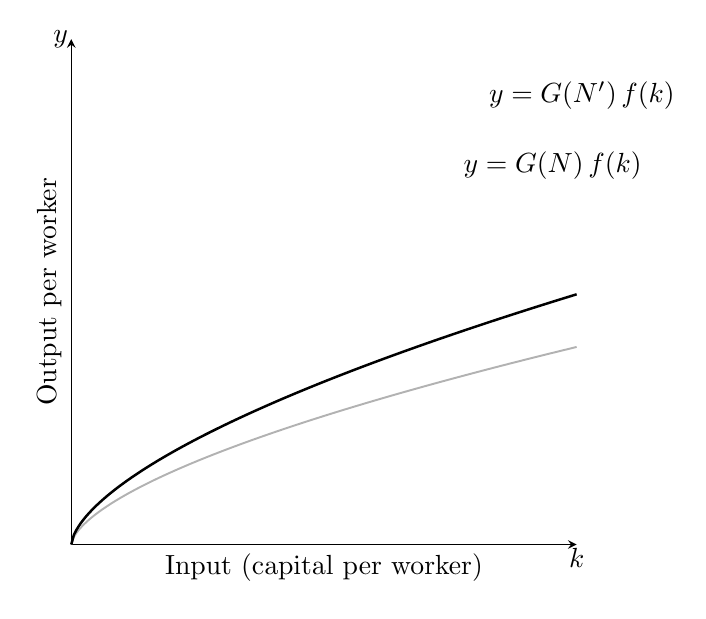
\begin{tikzpicture}
  \begin{axis}[
    width=8cm, height=8cm,
    xmin=0, xmax=10,
    ymin=0, ymax=8,
    axis lines=left,
    ticks=none,
    enlargelimits=false,
    clip=false,
    xlabel={Input (capital per worker)},
    ylabel={Output per worker},
    xlabel style={font=\normalsize},
    ylabel style={font=\normalsize},
  ]

    % 参数(可微调以匹配形状)
    \pgfmathsetmacro{\alpha}{0.62}
    \pgfmathsetmacro{\Alow}{0.75}
    \pgfmathsetmacro{\Aup}{0.95}

    % 下方曲线
    \addplot[curveLow, domain=0:10, samples=200]
      ({x},{\Alow*pow(x,\alpha)});

    % 上方曲线
    \addplot[curveUp, domain=0:10, samples=200]
      ({x},{\Aup*pow(x,\alpha)});

    % 轴端变量(贴近轴的末端)
    \node[labelText, anchor=east] at (axis cs:0,8) {$y$};
    \node[labelText, anchor=north] at (axis cs:10,0) {$k$};

    % 曲线标签(位置可微调)
    \node[labelText, anchor=west] at (axis cs:7.7,6.0)
      {$y=\GN\,f(k)$};
    \node[labelText, anchor=west] at (axis cs:8.2,7.1)
      {$y=\GNprime\,f(k)$};

  \end{axis}
\end{tikzpicture}
\end{document}